\chapter{はじめに}\label{sec:Introduction} % 章
\section{研究背景}\label{sec:Background} % 節

ここには研究の背景を書くが,せっかくなので\LaTeX の基本的な使い方について説明する.
実際に論文を提出するときは,この部分はすべて消去してあることを確認してほしい.

%%%% 項が変わるときには%を入れると可読性が増す
\subsection*{コンパイルできないときは}\label{sec:コンパイル}

ここでは,Dockerコンテナには正しく入れていると仮定して,\LaTeX の問題でコンパイルできないとき,コンパイルしたのにpdfに反映されていない場合を考える.その場合,以下の原因が考えられる.
\begin{itemize}
    \item 変更を保存していない.デフォルトでは自動保存されないため,ファイルを変更した際にはCtrl+Sで上書き保存を行う.変更したすべてのファイルで行うこと.
    \item 図や表が無い.指定したファイルが無い場合,コンパイルエラーが発生する.ファイルが存在するか,ファイル名(拡張子を含む)が間違っていないかを確認する.
    \item その他エラーが発生している.画面下部の「PROBLEMS」を確認し,対処する.また,まれに「PROBLEMS」には詳細なエラー内容が表示されないことがある.その場合は隣の「OUTPUT」を確認する.
\end{itemize}

%%%% 項が変わるときには%を入れると可読性が増す
\subsection{改行}\label{sec:改行}
改行したい場合は,ただ改行するのではなく,一行空ける.日本語の文章の場合は,段落の最初の1文字分が字下げされる.\\
もし字下げせずに改行したい場合は,バックスラッシュ(円マーク)をふたつ挿入する.

\vskip\baselineskip
空行を入れたい場合は行送りのコマンドを使う.

改行や空白も含めてそのまま出力させたい場合には,verbatim*を使う.
第\ref{sec:文字}項で説明する特殊文字もそのまま出力できる.
\begin{verbatim*}
verbatim*ブロック内では,改行や空白 がそのまま出力される
改行をいくつ入れても


反映
記号も出力 \verb*| ! " $ % $ & |  
\end{verbatim*}

%%%%
\subsection{文字の大きさ・色・フォント・特殊文字}\label{sec:文字}
部分的に文字サイズを変更したい場合は,{\tiny 小さい字}や{\large 大きい字}のように使う.あまり使わない.

また,文字色を変更したい場合は,定義されている色は\textcolor{lightcyan}{シアンの文字},定義されていない色は\textcolor[rgb]{0.0,0.0,1.0}{青色の文字}のように使う.

文字のフォントを変更したい場合は,\textrm{Roman},\texttt{TypeWriter}のように使う.

\% (percent),\{ (left brace),\} (right brace),\& (ampersand), \#(hash), \$(dollar), \textasciicircum(caret), \textasciitilde(tilde), \textbackslash(backslash), \_(underscore)は特殊文字のため,そのまま入力できないことに注意する.

%%%%
\subsection{ラベルと参照}\label{sec:ラベル}
章(chaper),節(section),項(subsection),目(subsubsection)には自動的に番号がつけられる.
別の章を引用する場合は,第2章,第3章,・・・と直接書くのではなく,ラベルを使って第\ref{sec:Introduction}章,第\ref{sec:RecentWorks}章,・・・と引用する.ラベルを使う場合は,一般には2回コンパイル(緑の矢印を押してbuildすること)しないと正しく反映されないので注意する.

また,参考文献を引用したい場合は,references.bibに引用元が記述されていることを確認し,次\cite{ref:mnih2013playing}のように引用する.

%%%%
\subsection{箇条書き}\label{sec:箇条書き}
番号付き箇条書きをする場合には,以下のように使う.
\begin{enumerate}
    \item ひとつめ
    \item ふたつめ
    \item みっつめ
    \begin{enumerate}
        \item 入れ子のひとつめ
        \item 入れ子のふたつめ
    \end{enumerate}
    \item[11] 見出しを変えることもできる 
    \item そのあとの項目は見出しを変える前のものに依存する
\end{enumerate}

番号なし箇条書きをする場合には,以下のように使う.
\begin{itemize}
    \item ひとつめ
    \item ふたつめ
    \begin{itemize}
        \item 入れ子のひとつめ
    \end{itemize}
\end{itemize}

%%%%
\subsection{数式の記述}\label{sec:数式}
数式を挿入する場合,インライン数式モード(文章中に数式を埋め込むモード)では$y=ax^{2}+bx+c$のように数式をドルマークで囲むことで挿入できる.文章中で変数の定義(ここで,$0<x<5$である.とか)をする場合によく用いられる.

ディスプレイ数式モード(数式をセンタリングして挿入するモード)ではいくつかの方法で挿入できる.
単純な挿入の場合,$$x=\frac{-b\pm\sqrt{b^{2}-4ac}}{2a}$$のようにドルマーク2つで囲むことで挿入できる.

しかし,可読性や余白,等号の位置などを踏まえて,一般にはalign環境を用いる.式変形を書き下す場合は,列を揃えてほしい記号の前にアンパサンドを入れる.
\begin{align}
	T &= T_{1} + T_{2} = \frac{1}{2}m_{1}\left(\dot x_{1}^{2} + \dot y_{1}^{2}\right) + \frac{1}{2}J_{1}\dot\theta_{1}^{2} + \frac{1}{2}m_{2}\left(\dot x_{2}^{2} + \dot y_{2}^{2}\right) + \frac{1}{2}J_{2}\left(\dot\theta_{1} + \dot\theta_{2}\right)^{2} \label{eq:T}\\
	U &= U_{1} + U_{2} = 0 \label{eq:U}\\
	F &= F_{1} + F_{2} = \frac{1}{2}\mu_{1}\dot\theta_{1}^{2}  + \frac{1}{2}\mu_{2}\dot\theta_{2}^{2} \label{eq:F}
\end{align}

式が長すぎて1行に収まらない場合は,nonumberとquadを用いる.
\begin{align}
	T &=  \frac{1}{2}m_{1}\left(\dot x_{1}^{2} + \dot y_{1}^{2}\right) + \frac{1}{2}J_{1}\dot\theta_{1}^{2} + \frac{1}{2}m_{2}\left(\dot x_{2}^{2} + \dot y_{2}^{2}\right) + \frac{1}{2}J_{2}\left(\dot\theta_{1} + \dot\theta_{2}\right)^{2} \nonumber\\
	%
    &= \frac{1}{2}m_{1}\left\{(-l_{1}\dot\theta_{1}\sin\theta_{1})^{2} + (l_{1}\dot\theta_{1}\cos\theta_{1})^{2}\right\} + \frac{1}{2}J_{1}\dot\theta_{1}^{2} \nonumber\\
    &\quad +\frac{1}{2}m_{2}\left[ \left\{ -L_{1}\dot\theta_{1}\sin\theta_{1} -l_{2}(\dot\theta_{1}+\dot\theta_{2})\sin(\theta_{1}+\theta_{2})\right\}^{2} + \left\{ L_{1}\dot\theta_{1}\cos\theta_{1} + l_{2}(\dot\theta_{1}+\dot\theta_{2})\cos(\theta_{1}+\theta_{2})\right\}^{2} \right] \nonumber\\
    &\quad + \frac{1}{2}J_{2}(\dot\theta_{1}+\dot\theta_{2})^{2} \label{eq:Tarray1}\\
    %
    &= \frac{1}{2}(m_{1}l_{1}^{2}\dot\theta_{1}^{2} + J_{1}\dot\theta_{1}^{2}) 
    + \frac{1}{2}\left[ m_{2}\left\{L_{1}^{2}\dot\theta_{1}^{2} + l_{2}^{2}(\dot\theta_{1}+\dot\theta_{2})^{2} + 2L_{1}l_{2}\dot\theta_{1}(\dot\theta_{1} + \dot\theta_{2})\cos\theta_{2}\right\} + J_{2}(\dot\theta_{1}+\dot\theta_{2})^{2}\right] \label{eq:Tarray}
\end{align}

%%%%
\subsection{図表の挿入}\label{sec:図表}

図表を挿入する場合,figureフォルダとtableフォルダのなかに図表を格納しておく.ただし,表はこのファイル内に直接記述することができるため,好きな方法を選んでほしい.

\vskip\baselineskip
表を挿入する場合は,表\ref{tab:labmem}のように使う.
\begin{table}[htbp]
    \centering
    \input{table/labmem.txt} % 表本体が記されたテキストファイル
    \caption{研究室メンバーの内訳} % 表の題名
    \label{tab:labmem} % 表のラベル(tab:から始めるとわかりやすい)
\end{table}

直接記述することもできる.
\begin{table}[htbp]
    \centering
    \begin{tabular}{|c|c|c|c|c|c|}
        \hline
        & \multicolumn{2}{|c|}{Docter, etc.} & \multicolumn{2}{|c|}{Master} & Bachelor\\\hline\hline
        Post & Asst. Prof. & D1 & M2 & M1 & B4\\\hline
        Number of people & 1 & 2 & 4 & 3 & 6\\\hline
    \end{tabular}
    \caption{研究室メンバーの内訳} % 表の題名
    \label{tab:labmem_direct} % 表のラベル(tab:から始めるとわかりやすい)
\end{table}

図を挿入する場合は,図\ref{fig:labpic}のように使う.
\begin{figure}[htbp]
    \centering
    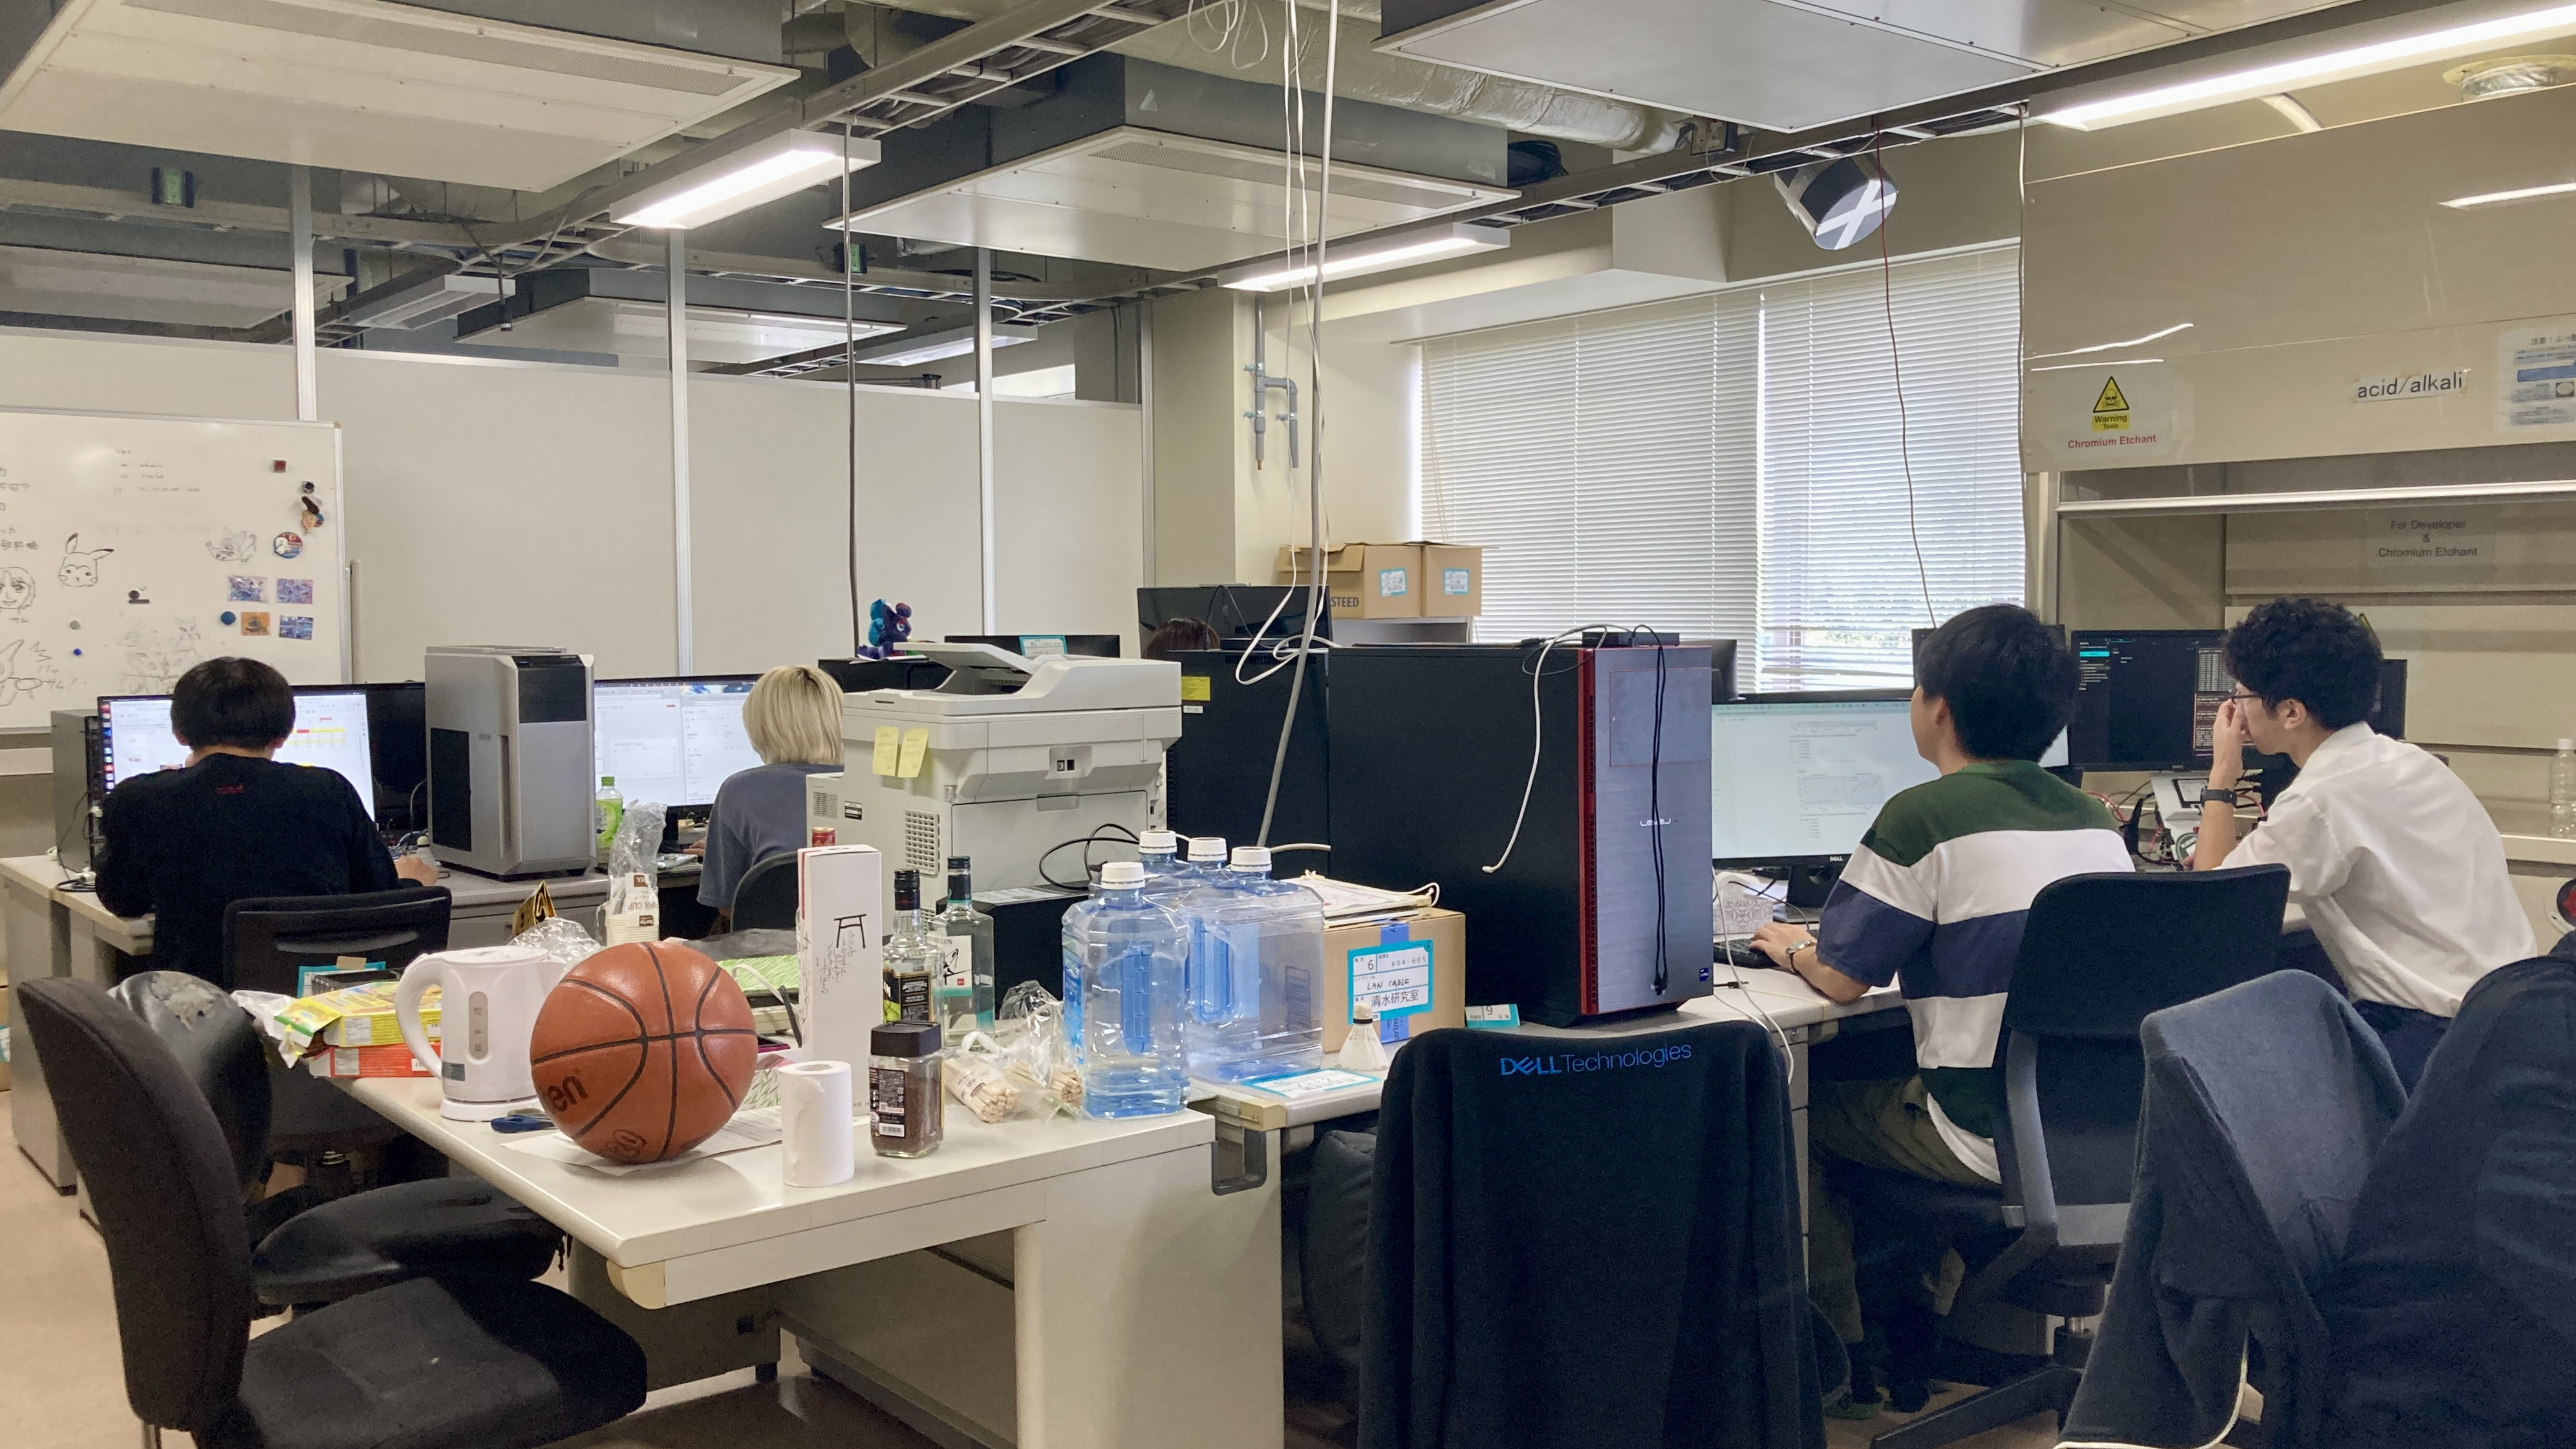
\includegraphics[width=.5\textwidth]{figure/labpic.jpg} % 紙面の横幅の0.5倍で図を挿入する
    \caption{研究室の様子} % 図の題名
    \label{fig:labpic} % 図のラベル(fig:から始めるとわかりやすい)
\end{figure}

図や表を並べて挿入する場合は,minipage環境を使う.また,[htbp]のところを[H]にすることで,強制的にここ(=here)に図を挿入できる.
\begin{figure}[H]
	\begin{minipage}{.5\textwidth}
        \centering
		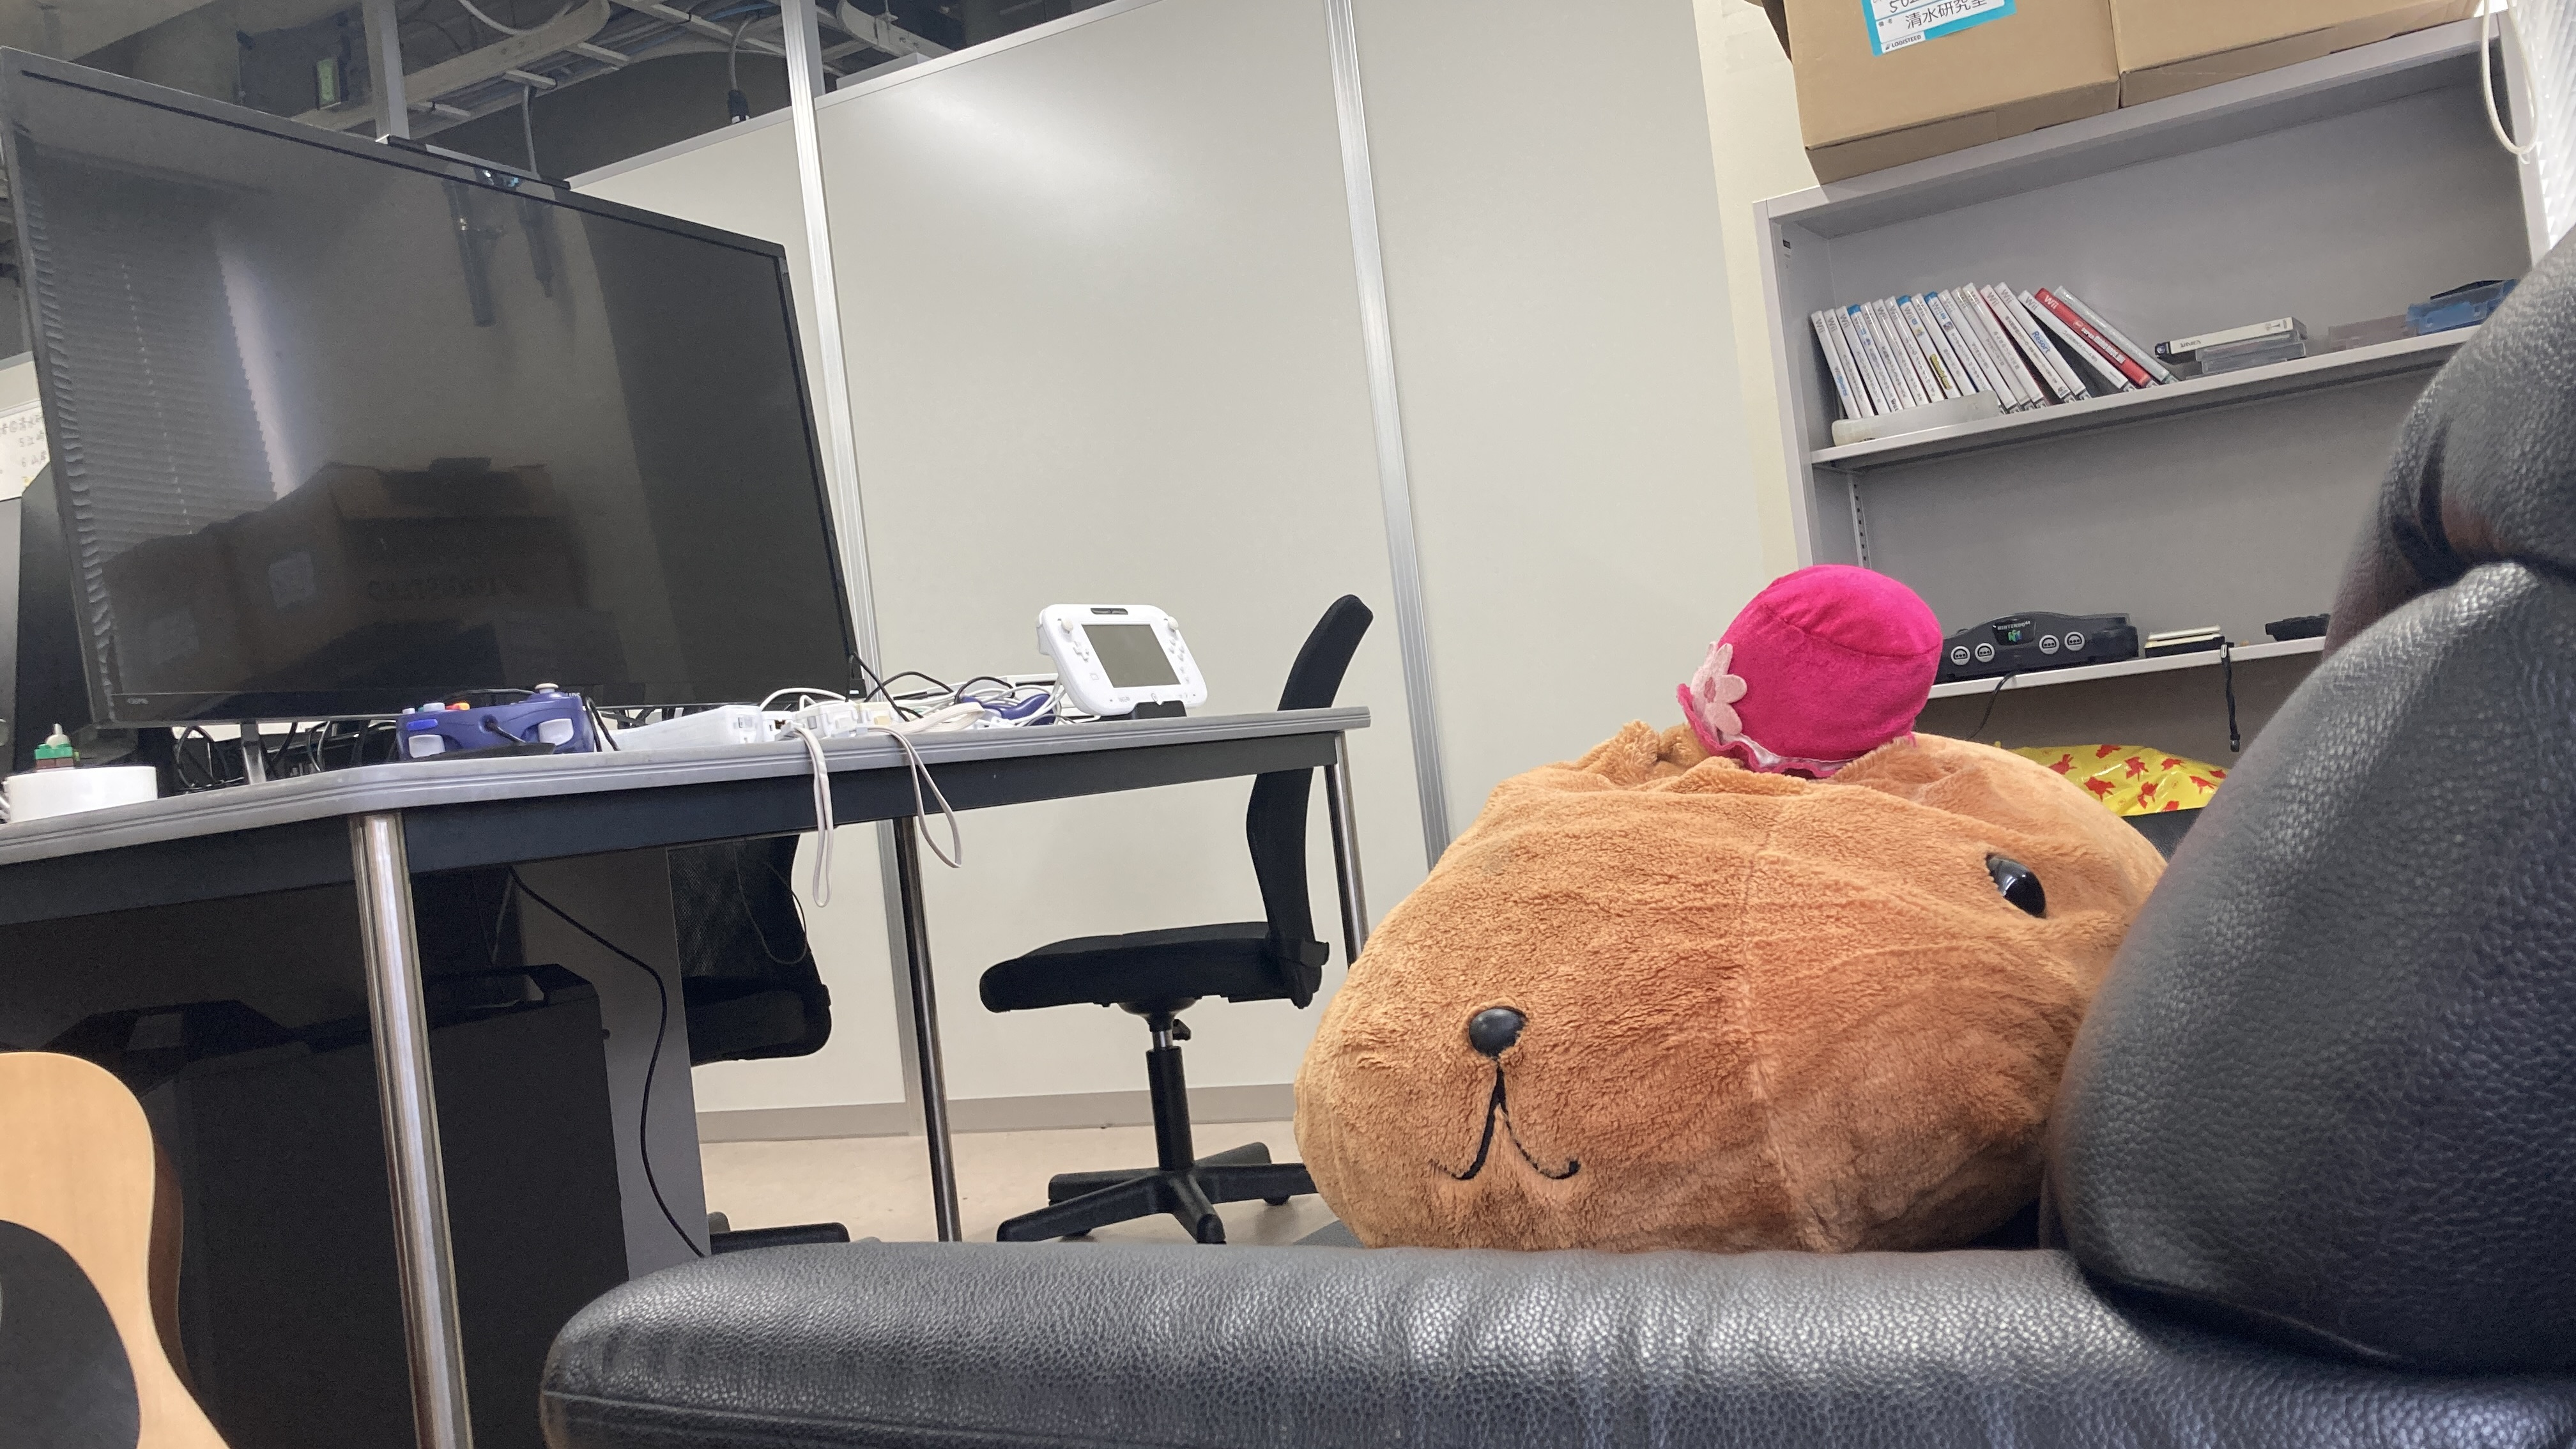
\includegraphics[width=.95\textwidth]{figure/labpic_game.jpg}
		\subcaption{ゲーム} % subcaptionを使うことで図1(a)のような表記が可能.使いたくなければcaptionに変更する
	\end{minipage}\hfill
 	\begin{minipage}{.5\textwidth}
        \centering
		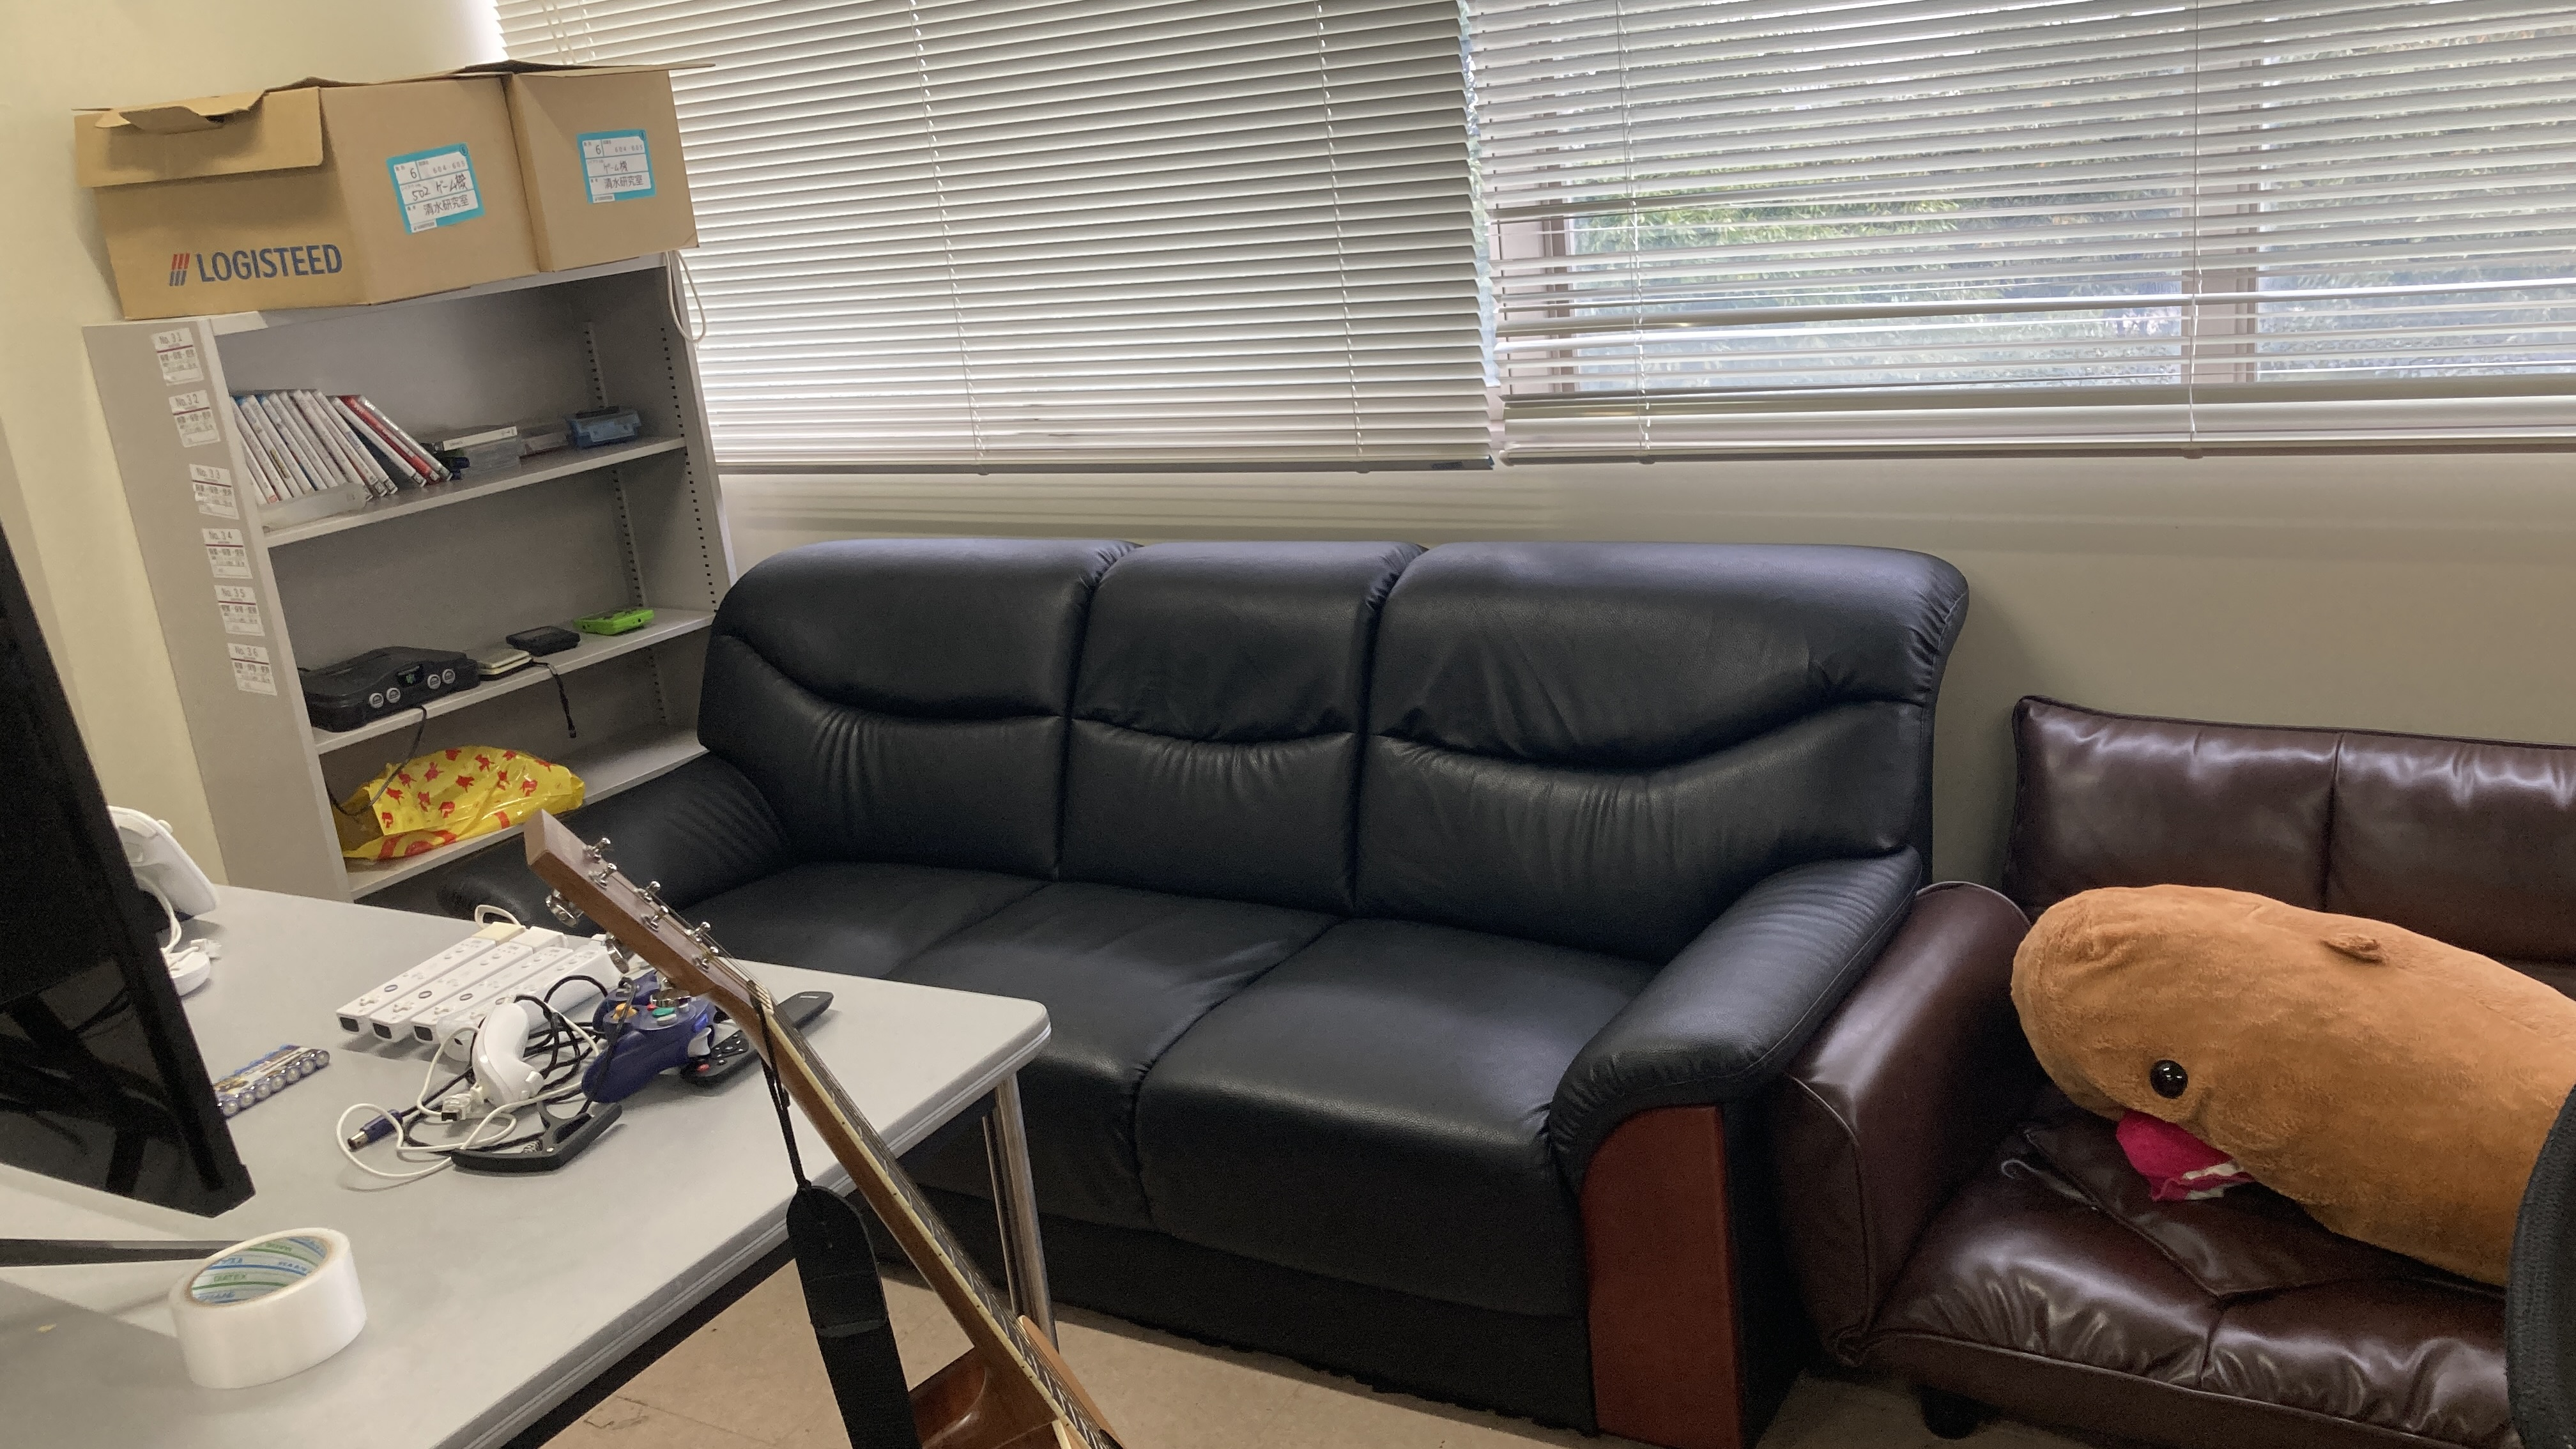
\includegraphics[width=.95\textwidth]{figure/labpic_sofa.jpg}
		\subcaption{ソファー}
	\end{minipage}\hfill
	\caption{研究室リフレッシュコーナーの様子}\label{fig:labpic_ref}
\end{figure}

章番号と同様に,ラベルを使うことで図\ref{fig:labpic},表\ref{tab:labmem}のように引用できる.ラベルはfig:fig1, fig:fig2,・・・のように通し番号にするのではなく,図そのものを説明するような名づけをする.

%%%%
\subsection{プログラムの挿入}\label{sec:program}
実際のプログラムの一部を(タブなども含めて)挿入したい場合は,リスト\ref{prog:hello}のように挿入する.
\begin{lstlisting}[caption=C言語で"Hello world!"を出力するプログラム,label=prog:hello]
    #include<stdio.h>
    int main(){
       printf("Hello world!");
    }
\end{lstlisting}

%%%%
\subsection{改ページ}\label{sec:改ページ}
改ページしたい場合は,clearpageを使う.
\clearpage

%%%%%%%%%%%%%%%%%%%%%%%%%%%%%%%%%%%%%%%%%%%%%%%%%%%%%%%%%%%%
\section{本論文の構成}\label{sec:本論文の構成}

ここに論文の構成を書く.

第\ref{sec:RecentWorks}章では,・・・

第\ref{sec:Method}章では,・・・

第\ref{sec:Experiments}章では,・・・

第\ref{sec:Conclusion}章では,・・・


